\documentclass[tikz]{standalone}

\usetikzlibrary{positioning}

\begin{document}
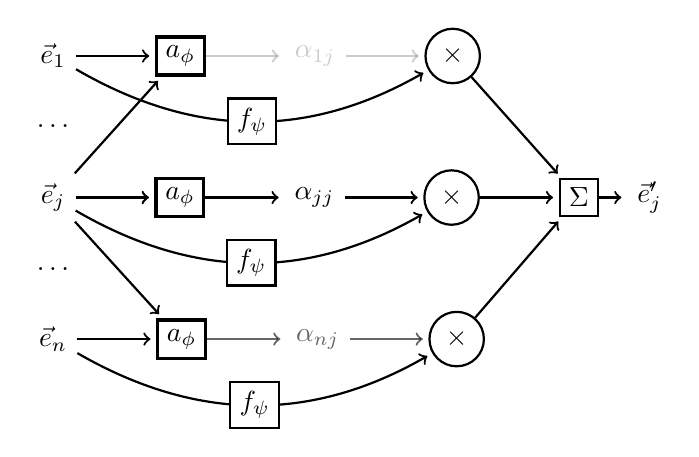
\begin{tikzpicture}[shorten >=2pt, thick, ->]

  \node (X1) {$\vec e_1$};
  \node[rectangle, below=3ex of X1] (x_dots_1) {$\dots$};
  \node[below=3ex of x_dots_1] (Xj) {$\vec e_j$};
  \node[rectangle, below=3ex of Xj] (x_dots_2) {$\dots$};
  \node[below=3ex of x_dots_2] (Xn) {$\vec e_n$};

  \node[rectangle, draw, very thick, right=of X1] (attn_1) {$a_\phi$};
  \node[rectangle, draw, very thick, right=of Xj] (attn_j) {$a_\phi$};
  \node[rectangle, draw, very thick, right=of Xn] (attn_n) {$a_\phi$};

  \draw (X1) edge (attn_1) (Xj) edge (attn_1);
  \draw (Xj) edge (attn_j) ([xshift=3em]Xj) edge (attn_j);
  \draw (Xj) edge (attn_n) (Xn) edge (attn_n);

  \node[right=of attn_1, opacity=0.2] (alpha_1j) {$\alpha_{1j}$};
  \node[right=of attn_j, opacity=1] (alpha_jj) {$\alpha_{jj}$};
  \node[right=of attn_n, opacity=0.6] (alpha_nj) {$\alpha_{nj}$};

  \node[circle, draw, right=of alpha_1j] (times_1) {$\times$};
  \node[circle, draw, right=of alpha_jj] (times_j) {$\times$};
  \node[circle, draw, right=of alpha_nj] (times_n) {$\times$};

  \node[rectangle, draw, right=of times_j] (sum) {$\Sigma$};

  \node[right=1em of sum] (x_tprim) {$\vec e_j'$};

  \draw[opacity=0.2] (attn_1) -- (alpha_1j);
  \draw[opacity=1] (attn_j) -- (alpha_jj);
  \draw[opacity=0.6] (attn_n) -- (alpha_nj);

  \draw (X1) edge[bend right] node[rectangle, draw, fill=white, midway] {$f_\psi$} (times_1);
  \draw (Xj) edge[bend right] node[rectangle, draw, fill=white, midway] {$f_\psi$} (times_j);
  \draw (Xn) edge[bend right] node[rectangle, draw, fill=white, midway] {$f_\psi$} (times_n);

  \draw (times_1) edge (sum) (times_j) edge (sum) (times_n) edge (sum);

  \draw[opacity=0.2] (alpha_1j) -- (times_1);
  \draw[opacity=1] (alpha_jj) -- (times_j);
  \draw[opacity=0.6] (alpha_nj) -- (times_n);

  \draw (sum) -- (x_tprim);

\end{tikzpicture}
\end{document}
